\documentclass[12pt, oneside, a4paper]{article}
\usepackage[spanish]{babel}
\usepackage[utf8]{inputenc}
\usepackage[colorlinks,bookmarksopen]{hyperref} % Para los enlaces web 
\usepackage{graphicx}
\usepackage{paralist} % Para las listas dentro de los párrafos tipo (i) esto (ii) lo otro
\title{Metapesca: Guía de Desarrollo}
\author{Versión 26.1.6}


\begin{document}
\maketitle

	\section{Estructura básica}

		METAPESCA es un modelo general para la dinámica poblacional y pesquera de una metapoblación de organismos bentónicos, compuesta por subpoblaciones conectadas entre ellas por dispersión larval. En su versión inicial, el modelo tenía algunos aspectos en común con un modelo de simulación utilizado por Botsford (1995) y Botsford et al. (1998) para explorar la dinámica de este tipo de recursos. Esos modelos fueron discutidos en detalle durante un taller conducido en octubre de 2001 en Valparaíso, del que participó el Prof. Botsford. El y su grupo los han aplicado específicamente a los stocks de erizo de California, así como en la exploración de estrategias rotativas y de los efectos de áreas marinas protegidas. Versiones ulteriores de METAPESCA incorporan explícitamente el proceso de pesca y el manejo.
		
		
		El código del modelo está escrito en VBA (Visual Basic for Applications) utilizando EXCEL como plataforma. 

		Tiene una estructura modular, consistiendo de los siguientes módulos principales que son llamados en cada iteración desde el módulo principal:

			\begin{enumerate}
				\item Recepción de nuevos “settlers” (procesos post-dispersión) \emph{M4\_CalcRecruits}.
				\item Producción y distribución de las larvas (dispersión, introducido mediante una matriz de conectividad) \emph{M6\_Prod\_Alloc\_Larvae}
				\item Estrategias de manejo (globales, espaciales, medidas temporarias) \emph{Management\_Procedure}
				\item Asignación del esfuerzo de pesca (\emph{M7\_Fishing}).						
				\item Dinámica de cada subpoblación bentónica (crecimiento, mortalidad, etc.) \emph{M5\_Popdyn}

			\end{enumerate}

		\subsection {Recepción de nuevos “settlers”}
			Este modulo describe los procesos locales post-dispersión operando en cada celda receptora. Se encuentra contemplada la implementación de mecanismos compensatorios (inhibición del asentamiento por parte de los residentes) y depensatorios (atracción o protección de larvas competentes por parte de los residentes).

		\subsection{Producción y distribución de larvas}

			La produccion larval esta afectada por  procesos locales pre-dispersión en cada celda emisora de larvas de la matriz espacial. Estos procesos incluyen mecanismos compensatorios (denso-dependencia en el crecimiento, y por ende en el output reproductivo) y depensatorios (denso-dependencia de las tasas de fertilización). En su forma inicial la produccion de larvas asume la forma general de una función stock-reclutamiento tipo Beverton-Holt, aunque en este caso la relación no describe un proceso cerrado (como en la teoría clásica) sino la relación entre estadíos sucesivos de un proceso abierto. Este tipo de relación es esperable cuando existe un balance entre compensación y depensación pre-dispersivas; fenómenos de este tipo han sido bien documentados en el caso de los erizos (Citas).

			El proceso de dispersión larval es introducido mediante una matriz de conectividad entre las celdas. Los elementos de la matriz pueden ser especificados uno a uno por el usuario, pero se contemplan algunos prototipos básicos: subpoblaciones cerradas, conectividad a través de áreas adyacentes, pool larvario común entre subpoblaciones, y el caso en que la probabilidad de dispersión entre la celda emisora y la receptora es alguna función de la distancia entre las mismas o su posición geográfica (ESPECIFICAR TIPOS DE MODELOS, ver OKUBO). En estos casos puede especificarse la fracción de larvas retenida en cada área y el resto es distribuido automáticamente en función del prototipo de metapoblacion elegido. También existe la opción de importar la matriz de conectividad desde un archivo externo, por ejemplo archivos de salida de modelos de circulación o a través de análisis de tasas de recuperación de áreas post-explotación.

		\subsection{Estrategias de manejo}

			Las estrategias de manejo utilizadas pueden ser  tanto globales, espaciales y temporarias.
Dentro de las globales estan implementadas cuotas anuales de captura  y esfuerzo. Las medidas espaciales incluyen el uso de reservas (o refugios reproductivos) y rotacion de areas. La rotacion de areas es caracterizada a travez de la determinacion de un numero o fraccion del area total explotada y una densidad minima de reapertura de areas. Las medidas temporarias incluyen cierres por biotoxinas, proteccion de areas con juveniles, contaminacion o variaciones en la calidad del recurso. Otra medida de manejo utilizable (no implementada aun) es el uso de tallas minimas de captura.

		\subsection{Asignación del esfuerzo de pesca}

			En la implementación de estrategias de manejo espacialmente explícitas es indispensable analizar el comportamiento de asignación espacial del esfuerzo por parte de los pescadores. El análisis básico utiliza como modelos de referencia (análogos a un modelo nulo) la bien conocida Ideal Free Distribution (IFD) y la asignación proporcional (modelo gravimétrico). Se ha explorado el rango de niveles de depleción en que ambas son aproximadamente equivalentes, y se prevé en el futuro incluir otras variantes del modelo gravimétrico (Caddy, 1975, Walters et al., 1993).

			Las variantes que se prevén incorporar incluyen matrices de distancias entre subpoblaciones (o procedencias) y “puertos” (sitios de partida, desembarque, comercialización), así como los costos operativos asociados; relaciones entre calidad del recurso y precio; costos de cambiar de lugar (“switching”); “suitability” de las áreas debida a factores distintos de las distancias (dependiente de las “utility functions” percibidas por los pescadores), etc.

			En determinadas situaciones no es necesario o practico modelar el esfuerzo, como el caso de la pesqueria de Geoducks en USA donde parcelas (tracks) asignadas a pesca son explotados hasta llegar a un umbral determinado, siendo irrelevante el patron de distribucion espacial del esfuerzo requerido para llegar a dicho umbral.

		\subsection {Dinámica de cada subpoblación bentónica}

			Dinámica de las subpoblaciones, incluyendo crecimiento y mortalidad. El crecimiento está modelado de forma recursiva, de manera de poder agregar denso-dependencia. El crecimiento compensatorio esta modelado mediante una funcion lineal en funcion de la fraccion de la capacidad de carga poblacional (K) en la que se encuentra cada subpoblacion y la fraccion del alfa maximo de crecimiento.

		\subsection{Esquema general}
		
			\begin{figure}[htb]
				\begin{center}
					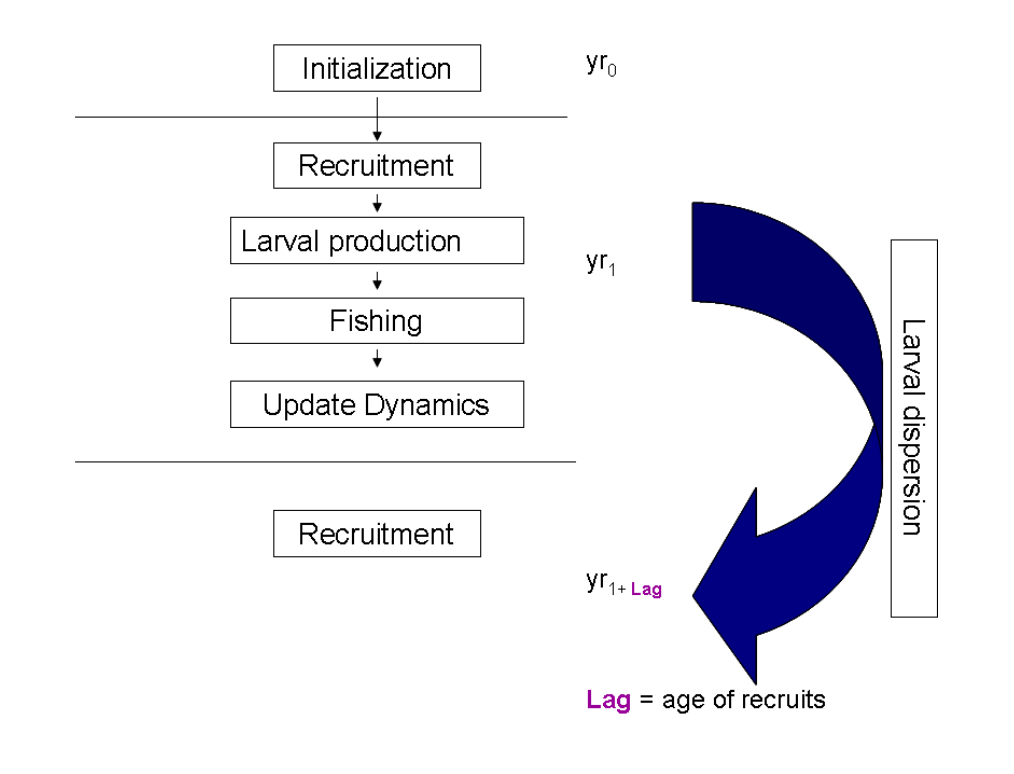
\includegraphics[width=\textwidth]{MetapescaDinamics.png}
					\caption{Esquema del orden de los eventos en el modelo.}
					\label{fig:Esquema general}
				\end{center}
			\end{figure}	
		
		El código incluye, además, módulos que agrupan la generación del output, gráficos y menús. 

		La siguientes son las principales variables de estado de la dinámica poblacional:
		\begin{enumerate}
			\item Numero de individuos a la edad, tiempo, procedencia.
			\item Talla a la edad, tiempo, procedencia.
			\item Biomasas desovante, explotable y total corregidas por variación de talla a la edad.
			\item Numero de huevos producidos por población.
			\item Numero de larvas asentándose por población.
		\end{enumerate}
 
 
		\subsection{Definiciones principales}
		
		\begin{description}
		\item[Áreas] Unidades espaciales mínimas del modelo.
		\item[Biological Region] Grupos de áreas que comparten parámetros de crecimiento y mortalidad. 
		\item[Regiones de manejo] Unidades espaciales de gestión. 		
		\end{description}
	\section{Simulación: Paso a paso}
	
		\subsection{Diagrama de secuencias: Flujo de ejecución}
		El módulo principal de la aplicación en Excel es \emph{M0\_Main} (Figura \ref{fig:FlujoEjecucion}), desde donde se llama a todos los módulos determinando la secuencia de ejecución de las distintas partes del modelo.

		\begin{figure}[htb]
		\begin{center}
			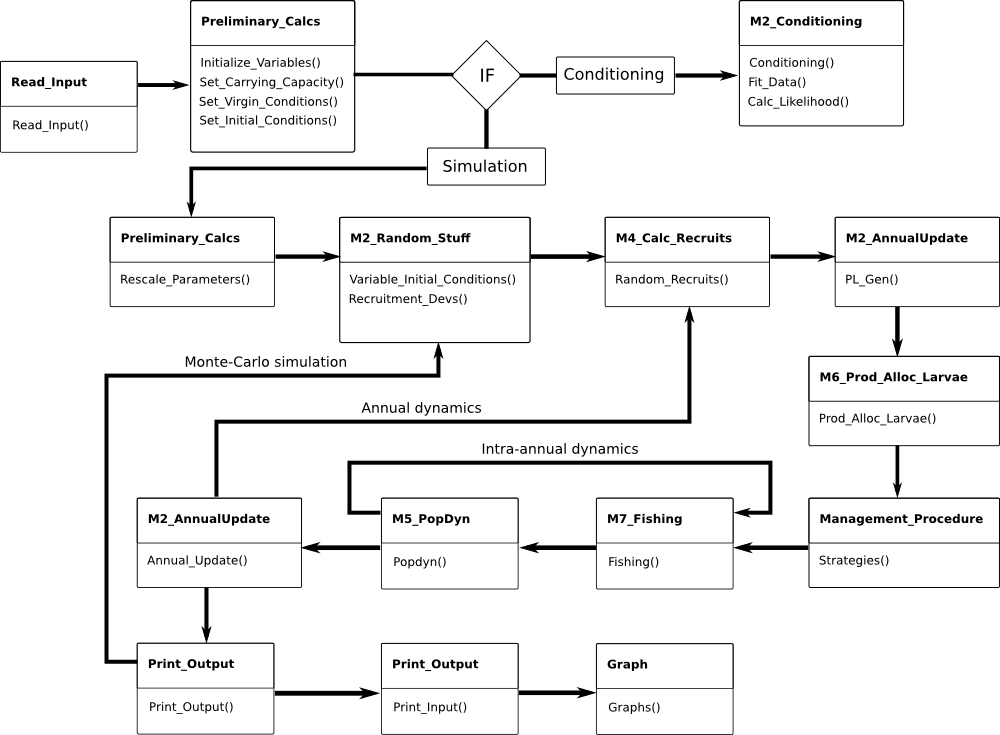
\includegraphics[width=\textwidth]{DiagramaMetapesca.png}
		\caption{Flujo de Ejecución del módulo principal de Metapesca.}
		\label{fig:FlujoEjecucion}
		\end{center}
		\end{figure}

		En primer lugar, se leen todas las variables de entrada llamando al módulo \emph{Read\_Input} y se almacenan en variables globales definidas en el módulo \emph{M1\_VarDef}. 
		Seguidamente se llama al módulo \emph{Preliminary\_Calcs} y se ejecutan los procedimientos que inicializan variables (\emph{initializeVariables()}), los que determinan las condiciones bajo las que estaría un población virgen no explotada (\emph{setVirginConditions()}) y las condiciones iniciales de las que va a partir el modelo (\emph{setInitialConditions()}). 
		Una vez realizados estos cálculos, hay una bifurcación en el modelo en función de si se quieren estimar los parámetros del modelo o realizar simulaciones. 
		Para ajustar el modelo a datos históricos se ejecuta \emph{M2\_Conditioning}. 
		Si se quieren llevar a cabo simulaciones se reescalan los parámetros (en función del intervalo de tiempo intra-anual elegido), se añade un componente aleatorio a las condiciones iniciales y se calculan las desviaciones del reclutamiento (módulo \emph{M2\_Random\_Stuff}). Allí se da inicio al ciclo anual. Éste comienza con el reclutamiento y la producción de larvas (módulo \emph{M6\_Prod\_Alloc\_Larvae}), que se distribuyen entre áreas de acuerdo a una matriz de conectividad. Luego sigue con el proceso de pesca (módulo \emph{M7\_Fishing}), el crecimiento y la mortalidad (módulo \emph{M5\_Popdyn}). Si la dinámica ocurre a una escala temporal menor que la anual (por ejemplo mensual), los módulos \emph{M7\_Fishing} y \emph{M5\_Popdyn} se repiten en los ciclos de dinámica intra-anual. 
		\par La pesca está regulada de acuerdo a reglas de manejo definidas en el procedimiento \emph{Strategies()} del módulo \emph{Management\_Procedure}.   
		Al final de cada ciclo anual, en la rutina \emph{AnnualUpdate()}, se calculan todos los totales de biomasas y se guardan las variables de abundancia a la edad, abundancia, talla y peso a la edad. 

		Una vez simulados todos los años se generan 'salidas' para todo el periodo de tiempo.
		Para cada una de las simulaciones de Monte Carlo a realizar se repite todo el proceso desde el cálculo de las condiciones iniciales variables y las desviaciones en el reclutamiento. 

		Al finalizar, se grafican los resultados.
		
		\subsection{Preliminary\_Calcs}
			\paragraph{Initialize\_Variables()}
				Subrutina. Inicializa las variables que son combinaciones de otras variables obtenidas en el Input. 
			\paragraph{Set\_Carrying\_Capacity()}
				Cálcula la composición poblacional en capacidad de carga. 
					\begin{enumerate}
						\item Distribuciones de tamaños: Asume que los individuos de cada clase de edad se distribuyen normalmente con media $\mu$ y desviación típica $\sigma$. Para el grupo 'Plus' se calculan el tamaño medio (ponderando los tamaños medios por edad por el número de individuos) y los porcentajes de cada tamaño (también ponderando por el número de individuos). 
						\item Abundancias y biomasa por edad. Asume que la población sólo pierde individuos por mortalidad natural ($N_{t+1}=N_t e^{-M}$)
						\item Reclutamiento: Calculo de la biomasa por recluta (BR0) para cada área y del reclutamiento vírgen ($R_0$) en base a la capacidad de carga (parámetro de entrada)bajo condiciones  
						\item Biomasa madura (para calcularla necesita la fracción de maduros (FracMat) y llama a \emph{M5\_Popdyn.Maturity()}) y biomasa vulnerable a la pesca. 
						\item Calcula la productividad (por unidad de biomasa desovante) de la población en condiciones vírgenes. 
						\item Imprimir condiciones de capacidad de carga en hoja de cálculo \emph{Carrying\_Capacity}. 
					\end{enumerate}
			\paragraph{Set\_Virgin\_Conditions()}
			Calcula las condiciones de equilibrio de la población virgen, que no son iguales a las de capacidad de carga si el aporte de larvas a alguna de las áreas está limitado. 
			Para ello realiza una simulación de 200 años partiendo de una población en capacidad de carga y escribe los resultados en la hoja \emph{Virgin\_Conditions})
			\paragraph{Set\_Initial\_Conditions()}
			Cuatro alternativas dependiendo del valor de \emph{RunFlags.Initial\_Conditions}: 
				\begin{enumerate}
					\item Población en capacidad de carga.
					\item Población en equilibrio sin explotar.
					\item Población explotada con tasa constante. Realiza una simulación de 200 años partiendo de una población vírgen y toma los valores finales como condiciones iniciales de la simulación. (Escribe las condiciones iniciales en \emph{Initial\_Conditions})
					\item Lee las condiciones iniciales desde archivo/hoja de cálculo (\emph{Initial\_Conditions}).
				\end{enumerate}
			Los tres primeros procedimientos escriben las condiciones iniciales en la hoja de cálculo \emph{Initial\_Conditions()} (el último no porque ya están ahí escritas).
				
			\paragraph{Rescale\_parameters()}
			Cambia la escala de la mortalidad natural, y parámetros de crecimiento anuales en función del número de intervalos temporales que hay dentro de un año (Nt).
		
			
			
		\subsection{M2\_Random\_Stuff}
			\paragraph{variableInitialConditions()}
				A partir de los valores iniciales se generan nuevos valores introduciéndoles un error multiplicativo $ln(\varepsilon) \in N(0,\sigma)$.
				 \par Bajo estas condiciones, el mejor estimador de la media es $e^{\mu+\frac{\sigma^2}{2}}$ y el mejor estimador de la mediana es $e^{\mu}$. La media va a variar en función de $\sigma$ mientras que la mediana es independiente de la varianza de los errores. 
				\par Por lo tanto, a fin de que la media de los reclutamientos simulados sea independiente de la variabilidad asumida, se trabaja con:
				$\varepsilon=e^{\mu-\frac{\sigma^2}{2}}$, 
				donde $\mu= Z\in N(0,1) \cdot \sigma$
				\par El mejor estimador de varianza en una log-normal es $\hat{S}^2=(e^{\sigma^2}-1)e^{2\mu+\sigma^2}$. Sabiendo que el coeficiente de variación $C_V=\frac{\hat{S}}{\bar{\varepsilon}}$, se cumple que en los casos en los que la varianza es pequeña (del orden de 0.x), $C_V \approx \sigma$. Por lo que en este caso se trabaja con los coeficientes de variación.
				\par Se calcula $N_t$ multiplicándolo por $\varepsilon$ y después se recalculan los Btotal, Bmature, Bvulnerable. Se reinician las variables temporales necesarias para comenzar las simulaciones (NTmp, BvulTmp, etc.). Se vuelve a hacer la survey parcial si procede llamando al procedimiento DoSurvey() y se le asignan al Atlas[ ] los valores de la evaluación. 
			
			\paragraph{recruitmentDevs()}
				Calcula las variaciones en el reclutamiento introduciéndoles correlación temporal según $\varepsilon_{t+1}= \rho \varepsilon_t + Y_t$ donde $Y \sim N(0, \sigma_{\varepsilon} \sqrt{1-\rho^2})$. 
				Asi $Y_t= \sigma_{\varepsilon} \sqrt{1-\rho^2} Z$.
				NOTA:Habría que hacer también correlaciones espaciales. Mirar como hacerlo con algebra de matrices.
				
			
		\subsection{M4\_Calc\_Recruits}
			Calcula el número de reclutas. Este módulo tiene tres procedimientos:\begin{inparaenum}[(i)] \item \emph{Deterministic\_Recruits()} se utiliza durante el cálculo de las condiciones vírgenes y de las condiciones iniciales bajo tasa de explotación constante, \item \emph{Random\_Recruits()} se utiliza durante las simulaciones de Monte-Carlo, \item \emph{Tunned\_Recruits()} toma índices de reclutamiento de un archivo (se utiliza en el conditioning) \end{inparaenum}.
			Dentro de estos tres procedimientos hay dos opciones: 
					\begin{enumerate}
						\item Reclutamiento constante. 
						\item Compensacion lineal.
					\end{enumerate}
			Estas opciones van ser muy similares en los dos primeros procedimientos, diferenciándose sólo en si se les añade o no un error. Calculan el número de reclutas, a partir del los \emph{settlers} (número de individuos que se asientan), y los van a pasar al número de invididuos de la primera clase de edad. Con esto se recalculan las biomasas totales (madura, vulnerable, total).
			\paragraph{Random\_Recruits()} 
				Dos opciones: 
					\begin{enumerate}
						\item Reclutamiento constante: $N_{t,i,edadinicial}= R_0 \cdot e^{Rdev-0.5 RecCV^2}$.
						\item Compensación lineal: $N_{t,i,edadinicial}=Settlers \cdot e^{Rdev-0.5 RecCV^2} $. Y está limitado a ser menor o igual que el menor de la $\frac{K - Btotal}{w_0}$ (condicionado a ser igual o mayor que cero) y el reclutamiento máximo que puede albergar el área($RMax$).
					\end{enumerate}
				
			
		\subsection{M2\_Annual\_Update.pLgen()}
			\paragraph{pLgen()}
				Genera los pL[], es decir el porcentaje de individuos de cada talla que hay en la población
		\subsection{M6\_Prod\_Alloc\_Larvae}
			\paragraph{Prod\_Alloc\_Larvae()}
				Calcula las larvas para cada año ($Bmature[year, area]* ProdXB$) y las reparte de acuerdo a la matriz de conectividad. Estas corresponden al número de individuos que llegan a cada área para asentarse en el año $t+Stage$, es decir después de que pase el suficiente tiempo como para que se recluten.  
				NOTA: Los settlers desde \emph{t=Año de Inicio} hasta \emph{t=(Año de inicio + Edad de reclutamiento-1)} ya se han calculado dependiendo de las condiciones iniciales de las que se parten. 
		\subsection{Management\_Procedures}
			\paragraph{Strategies()}
			Este procedimiento es el encargado de realizar las surveys (globales o parciales) si procede, de pasar las áreas a pescar a estado 'Abierto' (ClosedArea = False), y de generar un vector temporal(\emph{ClosedAreaTemp}) que especifica si dichas áreas están cerradas o abiertas y que le sirve de input al método \emph{Fishing()}. Además, ajusta la HarvestRate en caso necesario (que implicaciones en el manejo conllevaría esto, i.e., el hecho de que tengas que ajustar la harvest rate para no pasarte de los límites, ¿qué implicaría en el caso real?).
				Tres estrategias distintas:
					\begin{enumerate}
						\item Rotaciones. 
							\begin{enumerate}
								\item Se cierran todas las áreas a la pesca. 
								\item Si hay cuotas de captura.
									\begin{enumerate}
										\item Si hay feedback se realizan las evaluaciones de las áreas o, en el caso de que sean evaluaciones parciales, se calcula la cuota multiplicando la abundancia estimada por la harvest rate.
										\item Se van abriendo las áreas que cumplen la condición de reapertura (si hay, sino por orden).
										\item Se calculan el número de áreas que se van a pescar (Nfishedareas).
										\item Si la captura esperada sobrepasa la cuota se ajusta la HR. 
									\end{enumerate}
								\item Si hay cuotas de esfuerzo: No hace nada porque aún no se ha implementado. 
								\item Si es por tasas de explotación: Se hace abriendo sólo el porcentaje de la supercifie explotable que se correspondería con la harvest rate objetivo. 
								\begin{enumerate}
									\item Se abren las áreas que se van a pescar.
									\item Se cuenta cuantas son (Nfishedareas).
								\end{enumerate}
							\end{enumerate}
						\item Gestión por área
							\begin{enumerate}
								\item Si hay feedback se realizan las evaluaciones de las áreas (llamando a \emph{DoSurvey()}), y:
								\begin{enumerate}
									\item Si hay cuotas de captura: Se calculan las TACs por área (\emph{TAC\_area}).
									\item Si hay cuotas de esfuerzo: Hay que implementar una rutina que te calcule los \emph{TAE\_area[]}.
								\end{enumerate}
							\end{enumerate}
						\item Gestión regional
							\begin{enumerate}
								\item Si hay feedback se realizan las evaluaciones de las áreas (llamando a \emph{DoSurvey()}), y:
								\begin{enumerate}
									\item Si hay cuotas de captura: Se calculan las TACs por región (\emph{TAC\_region[]}).
									\item Si hay cuotas de esfuerzo: Hay que implementar una rutina que te calcule los \emph{TAE\_region[]}.
								\end{enumerate}
								\item Se calculan los EffortPulse (para el caso de TAEs y el resto). 
							\end{enumerate}
					\end{enumerate}
			Para todos los casos se calcula al final de la rutina los \emph{ClosedAreaTmp} para todas las áreas, que se le pasan al \emph{Fishing()}.
				
		\subsection{M7\_Fishing}
			\paragraph{Fishing()}
				Realiza las extracciones para cada pulso de pesca, calculando las capturas anuales por área. 
				Tres casos:
				\begin{enumerate}
					\item Rotaciones. Mira si el área está abierta, ajusta las tasas de explotación si es necesario, si hay survey parcial ajusta los Atlas y después calcula las capturas. 
					\item Por Área. Mira si las áreas están abiertas a la pesca, y si lo están:
						\begin{enumerate}
							\item Si hay cuotas de captura: Calcula la harvest rate, y después las capturas (si la harvest rate es mayor que 0.9 se toma como 0.9 y de ahí se sacan las capturas. 
							\item Si hay cuotas de esfuerzo: Entonces la $HR=1-e^{-Q(Area)*TAE}$ y de ahí se calculan las capturas.
							\item Si es por tasa de explotación: Se calculan las capturas a partir de esa tasa. 
						\end{enumerate}
					\item Por Región
					 \par Si es por harvest rate el programa no permite hacerlo, ya que considera que es análogo al caso de manejo por áreas y que debes utilizar esa opción. Sale un mensaje de aviso.
					\par Se va a poder realizar la distribución de la pesca entre áreas mediante varias estrategias, determinadas por el valor de \emph{EffortDistributionFlag}:
					\begin{enumerate}
						\item Ideal Free Distribution según el algoritmo 'obsoleto' o mediante la repartición del esfuerso en trozos o cachitos. 
						\begin{enumerate}
							\item Si hay cuotas de captura: IFD hasta que se llegan a las distintas cuotas por región.
							\item Si hay cuotas de esfuerzo: IFD dentro de cada región, para repartir ese esfuerzo entre áreas. 	 
						\end{enumerate}
						\item Ideal Free Distribution basada en el algoritmo de Walters \& Martell (2003). 
						\begin{enumerate}
							\item Si hay cuotas de esfuerzo: Se aplica el algoritmo de Walters para cada región y se reparten los esfuerzos calculados homegéneamente a lo largo de toda la temporada de pesca. NOTA: Con esto se podría jugar mirando que estrategias de repartición del esfuerzo a lo largo del año serían mejores (e.g. pescarlo todo al principio o esperar al final).
							\item Si hay cuotas de captura: En ello. Está implementado para el caso en el que haya una única región. 
						\end{enumerate}
						\item Gravitacional (No implementada)
					\end{enumerate}

				\end{enumerate}
		\subsection{M5\_Popdyn}
			Este módulo se encarga de hacer crecer y morir (mortalidad natural) a los individuos. 
		
				\paragraph{PopDyn()} Se determina la g (fracción de reducción) del crecimiento. 
				Si una edad no está reclutada o está parcialmente reclutada, se calcula en dónde se encuentra con respecto a la talla vulnerable (estándarizando y mirando la probabilidad equivalente de una $N(0,1)$. Si empieza a ser vulnerable Flag\_Rec\_Fish pasa a ser 2 y si ya es totalmente vulnerable 3.  
		
				El crecimiento puede se linealmente dependiente o independiente.
				Flag\_Rec\_Fish puede tener tres valores. 1 (por defecto) indica que la edad no ha sido reclutada. 2 que ha sido parcialmente reclutada y 3 que está totalmente reclutada. Según el estado de cada edad, se va a llamar a Norm (no reclutada) o Trunc\_Norm (el resto de casos) para determinar la estructura de tallas de cada edad. 
				
				La clase de edad AgePlus se calcula de forma diferente, haciendo crecer los distintos intervalos de talla y asignando a esos individuos a su clase de talla final correspondiente. Así, se calcula para cada intervalo de talla un Lplus que se corresponde con el tamaño que tendrían los individuos de esa talla después de crecer, y se mira en que intervalo de tallas quedarían.  
				
				Se calculan las FracSel, biomasas y pesos para el intervalo de tiempo siguiente. 
				
				Como la biomasa cambia al crecer los individuos, hay que controlar que no se sobrepase la capacidad de carga del medio, y en el caso que se sobrepase aumentar la mortalidad. Al tratarse de un modelo discreto, si se espera a que se llegue a capacidad de carga para aumentar la mortalidad, se van a generar ciclos de reclutamiento-no reclutamiento (ya que cuando llega a capacidad de carga no hay sitio para más individuos y no habría reclutamiento), para 'suavizar' este proceso y adecuarlo más al caso diferencial, lo que se hace es asumir que hay una capacidad de carga de adultos de la forma:
				\begin{equation}
					K_{adultos}= K - R_0 Peso_{inicial}
				\end{equation}
				  
				 Donde $K$ es la capacidad de carga del medio, $R_0$ es el reclutamiento en condiciones vírgenes (donde se asume que la población está en equilibrio, y el reclutamiento es el mínimo necesario para sustentar a la población y que este equilibrio se mantenga), y $Peso_{inicial}$ es el peso medio por recluta. 
				 
				 Partiendo de esta $K_{adultos}$ se calcula la mortalidad extra que hay que aplicarle a la población en el caso de que esta capacidad de carga se vea sobrepasada, de tal forma que:
				\begin{equation}
					XtraM= \frac{K_{adultos}}{B_{total}} 
				\end{equation}
				 XtraM sería la reducción en la supervivencia de los individuos si la $K_{adultos}$ se sobrepasa. Y esta se multiplica por la BtotTmp, BvulTmp y NTmp.
				
		\subsection{M2\_AnnualUpdate}
			\paragraph{AnnualUpdate()} Actualiza las variables temporales y las mueve de un año al siguiente. 
			
		\subsection{Print\_Output}
			\paragraph{printOutput()} Imprime los resultados de la simulación en las hojas de cálculo correspondientes.
			
		\subsection{Graphs}
			\paragraph{Graphs()} Se encarga de crear los gráficos de salida. En concreto:
				\begin{enumerate}
					\item Catch vs. Time
					\item Effort vs. Time
					\item Vulnerable biomass vs. Time
					\item Spawning biomass vs. Time
					\item Larvae vs. Time
					\item Density vs. Time
					\item Recruits vs. Time
					\item Total biomass vs. Time
					\item Harvest Rate vs. Time
					\item Depletion en la biomasa vulnerable vs. Time
					\item Depletion en la biomasa de maduros vs. Time
				\end{enumerate}
		
		
		

	\section{Library Functions}
	
	\paragraph{Norm(Area, Age)} Calcula las probabilidades que tendría cada clase de talla según una normal $N(\mu, \sigma)$. Como las clases de talla son valores discretos se divide cada probabilidad entre el sumatorio de todas ellas, para que la distribucion de las probabilidades vaya de $0$ a $1$.
	\paragraph{Cumd\_Norm(x)} Calcula la probabilidad acumulada desde $-\infty$ a $x$ según una $N(0,1)$.
	\paragraph{Trunc\_Norm(Area, age)} Calcula las probabilidades que tendría cada clase de talla según una normal $N(\mu, \sigma)$, truncando la función en los puntos en los que hay discontinuidades debido a los pulsos de pesca.

	\section{Variables del Programa}		

		
		\begin{description}
		% -- A -- %
		
		\item[Abundancetype] 1. Absoluta 2. Relativa CONTROL
		\item[AgeFullMature] Clase de edad a la que maduran los individuos (knife-edge). CONTROL
		\item[AgePlus] Grupo de edad que incluye a todos los individuos mayores que esa.
		\item[Alpha[Nareas]] $(1-e^{-k}) L_{inf} gk$ Primer término de la ecuación de crecimiento individual.
		\item[Alpha0[Narea]] Alpha
		\item[Amax[Nareas]] Edad máxima. (Inicializada en 1000. Comentado: -Log(0.0001)/M[Area]).
		\item[Atlas[Nareas]] Biomasa vulnerable estimada de todas las áreas. Utilizada en el caso de surveys parciales. No se estiman las abundancias de todas las áreas al mismo tiempo. 
		\item[aW[Nareas]] Multiplicador de la relación Talla-Peso (L-W).
		
		% -- B -- %
		\item[Beta[Nareas]] $1-(1-Rho) gk$ Segundo término de la ecuación de crecimiento individual.
		\item[Beta0[Narea]] Beta
		\item[Bg0[Nareas]] $\frac{k-B_{th}}{1-g_k}+B_{th}$
		\item[Bmature[Nareas, Nyears]] 
		\item[Bregion[Nareas]] Grupos de áreas que comparten los parámetros de crecimiento y mortalidad natural. Vector con el ID de la región biológica a la que pertenece cada área. 
		\item[BthThreshold[Nareas]] Biomasa de inicio de la denso-dependencia en \% de capacidad de carga.
		\item[Bmature[Nyears, Nareas]] Biomasa en estadío reproductivo maduro.
		\item[Btotal[Nyears, Nareas]] Biomasa total por área.
		\item[BtotTmp[Nareas]] Biomasa total por área. (Variable auxiliar utilizada en cálculos intra-season).
		\item[Bvulnerable[Nyears, Nareas]] Biomasa vulnerable por área. 
		\item[BvulTmp[Nareas]] Biomasa vulnerable por área. (Variable auxiliar utilizada en cálculos intra-season).
		\item[BR0] Biomasa en condiciones vírgenes por recluta(Se utiliza para el cálculo de la R0 en el reclutamiento). 
		\item[Bvultype] 1. Absoluta 2. Relativa CONTROL
		\item[bW[Nareas]] Exponente de la relación Talla-Peso (L-W).

		
		% -- C -- %
		\item[Candidate\_areas[Nregions, MaxNareas\_Region]] Matriz que contiene las áreas abiertas a la pesca para cada región (ordenadas, si procede, en función del tiempo de descanso que han tenido). Estas áreas se escriben en la hoja \emph{Calcs}.
		\item[Catch[Nareas, Nyears]]
		\item[ClosedArea[Styear, Nareas]] Variable booleana. ¿Área cerrada? Read\_Input sólo inicializa los valores para el primer año,\emph{iniciateVariables()} inicializa los valores para todos los años de las áreas cerradas permanentemente.
		\item[ClosedRegion[Nregions]] Variable booleana. ¿Región cerrada? Se actualiza anualmente.
		\item[ClosedRegionTmp[Nregions]] Variable booleana. ¿Región cerrada? Se actualiza en cada periodo de pesca intra-anual.		
		\item[Connect[Nareas, Nareas]] Matriz de conectividad larvaria.
		\item[CVmu[Nareas]] Coeficiente de variación de la talla media para cada clase de edad.
		
		% -- E -- %
		\item[EffortDistributionFlag] Distribución del esfuerzo. 1.Ideal Free Distribution 2. Gravitacional (Comentada en el código). CONTROL
		
		% -- F -- %
		\item[Feedback] Variable booleana ¿Hay una feedback control rule? CONTROL
		\item[Flag\_Rec\_Fish[Nareas,Nages]] Toma valor 1 en Preliminary\_Calcs. Se utiliza en popdyn(). 1 (por defecto) indica que la edad no ha sido reclutada. 2 que ha sido parcialmente reclutada y 3 que está totalmente reclutada.
		\item[frac[Nareas, Nages, NpulsosMax]] Toma valor 1 en Preliminary\_Calcs. Indica la fración de la población que es extraída en cada pulso de pesca.
		\item[FracMat[Nage]] Matriz con 1s y 0s para indicar qué edades son maduras y cuales no. 
		\item[FracSel[Nareas, Nages]] Proporción de la población que puede ser extraída por pesca para cada edad. 
		   
		% -- G -- %
		\item[g[Nareas]] Fracción de reducción de crecimiento cuando hay efectos densodependientes. Con este valor se calculan las Alphas y Betas para hallar la talla.
		\item[gk[Nareas]] Fracción de reducción de crecimiento en capacidad de carga (Si es denso-independiente es 1).
		\item[Growth\_type] Tipo de crecimento: 1. Denso-independiente; 2. Densodependiente. CONTROL
		
		% -- H -- %
		\item[HR\_start[Nareas]] Tasa de explotación inicial.
		\item[HRTmp[Nareas]] Tasa de explotación instantánea.
		\item[Hstrategy] Estrategia de explotación. 1. Rotacional; 2. Por área; 3. Por región. CONTROL
		
		% -- I -- %
		\item[IDopenarea[]] Vector que indica el índice de las áreas que están abiertas. Si hay que tener en cuenta el periodo de descanso (RestingTimeFlag) las ordena por periodo de descanso decreciente. (Variable Local - M7\_Fishing).
		\item[iLfull[Nareas]] Edad a la que los individuos se vuelven vulnerables a la pesca. 
		\item[Initial\_Conditions] 1. Inicio a capacidad de carga K; 2. Inicio bajo condiciones de explotación con una tasa determinada; 3. Leer condiciones de inicio desde archivo. CONTROL
		\item[InitialCV]
		\item[InputAbundance] Variable booleana. ¿Cargar información de abundancia desde archivo (Hoja de Metapesca)? CONTROL
		\item[InputBvul] Variable booleana. ¿Cargar información de biomasa vulnerable desde archivo (Hoja de Metapesca)? CONTROL
		\item[InputCatch] Variable booleana. ¿Cargar información de capturas desde archivo (Hoja de Metapesca)? CONTROL
		\item[InputRec] Variable booleana. ¿Cargar información de reclutamiento desde archivo (Hoja de Metapesca)? CONTROL
		
		% -- K -- %
		\item[k[Nareas]] Tasa de crecimiento individual (von Bertalanffy)
		\item[kcarga[Nareas]] Capacidad de carga. Aunque en el Input se introduce por $m^2$ al inicializar las variables se recalcula la total por área.
		
		
		% -- L -- %
		\item[l[Nilens]] Talla media para cada intervalo. Intervalos de talla definidos desde l(ilen)-Linc/2 hasta l(ilen)+Linc/2. 
		\item[L1] Tamaño inicial correspondiente a la edad inicial.
		\item[$\lambda$\_ProdxBiomasa] Productividad de la población. CONTROL
		\item[Lat[Nareas]] Latitud en grados decimales a la que se encuentra el área (Sólo para gráficos) ¿Cómo se define? ¿Punto medio del área? 
		\item[Lfull[Nareas]] Talla mínima de pesca (knife-edge).
		\item[Linc] Incremento de tamaño entre clases de tamaño. 
		\item[Linf[Nareas]] Tamaño máximo que pueden alcanzar los individuos (von Bertalanffy)
		\item[Long[Nareas]] Longitud en grados decimales a la que se encuentra el área.
		
		% -- M -- %
		\item[M[Nareas]] Mortalidad natural
		\item[MaxEffort] Esfuerzo máximo posible global. 
		\item[MaxNareas\_Region] Máximo del número de áreas abiertas a la pesca por región. 
		\item[mu[Nyears, Nareas, Nages]] Tamaño medio esperado para cada clase de edad. El tamaño inicial se corresponde con el esperado para el modelo de von Bertalanffy ($L_{inf}(1-e^{-k (t-t_0)})$)
		\item[muTmp[Nareas, Nages]] mu. Tamaño medio esperado para cada clase de edad.
		   
		
		% -- N -- %
		\item[N[Nyears, Nareas, Nages]] Número de individuos. (Nota: Al inicializar el vector en \emph{Virgin\_Conditions()} es por recluta pero por el medio pasa a ser número de individuos).
		\item[Nages] AgePlus - Stage + 1
		\item[Nareas] Número de áreas.
		\item[Nareas\_region[Nregions]] Áreas abiertas a la pesca de cada región. 
		\item[NBregions] Número de regiones biológicas.
		\item[Ndias\_before\_switch] Mínimo de días que tienen que pasar desde que se comienza a explotar un áreas hasta que puede cambiar de área.
		\item[Nfracs[Nages]] Número de fracciones (o truncaciones) que tiene la distribución de tallas por edad al verse sometida parcialmente a la pesca. Se inicializa en cero (quiere decir que la distribución no está truncada), y en PopDyn() va cambiando.
		\item[Nilens] Número de clases de talla (No es igual al número de clases de edad).
		\item[Nopenareas] Número de áreas abiertas a la pesca. 
		\item[NPulses] Pulsos de pesca (Es el número máximo de cambios que puede haber en un año). $365/(N_t*Ndias_{beforeswitch})$.
		\item[NpulsosMax] Nt*Nages Número de pulsos de pesca a los que se puede ver sometida una cohorte.
		\item[Nregions] Número de regiones de manejo.
		\item[Nreplicates] Número de simulaciones de Monte-Carlo a realizar. 
		\item[Nsurveys] Número de evaluaciones utilizadas para determinar el procedimiento de manejo????
		\item[Nt] Número de intervalos temporales en los que se divide el año.
		\item[Nt\_Season] Número de unidades de tiempo que dura la temporada de pesca. 
		\item[Nyears] Número de años ($Anho_{Final}-Anho_{Inicial}+1$).
		
		
		% -- O -- %
		\item[ObsError\_Survey] Error de observación de la evaluación. 1. Determinístico; 2. Estocástico. CONTROL
		\item[ObsAbundance[FilasHoja, 4]] Abundancia observada. Se cargan las 4 columnas (Year, Area, Index, CV) de \emph{ObsAbundance}.
		\item[ObsBvul[FilasHoja, 4]] Índice de biomasa vulnerable observada. Se cargan las 4 columnas (Year, Area, Index, CV) de \emph{ObsBvul}.
		\item[ObsCatch[Nyears, Nareas]] Capturas observadas (se obtienen de la hoja \emph{ObsCatch})
		\item[ObsRec[Nyears, Nareas]] Reclutamiento observado (se obtiene de la hoja de cálculo \emph{ObsRec})
		\item[Output\_Nage\_Nsize] Variable booleana. ¿Qué hace??? CONTROL
		\item[Output\_Size\_W] Variable booleana. ¿Qué hace?? CONTROL
		
		% -- P -- %
		\item[PartialSurveyFlag] Variable booleana. ¿Se hace sólo evaluación parcial? CONTROL
		\item[pL[Nyears, Nareas, Nilens]] Porcentaje de individuos de cada clase de talla que hay en la población.
		\item[pLage[Nareas, Nages, Nilens]] Porcentaje de individuos de la misma clase de edad para cada clase de talla. Siguen una distribución normal de esta forma ($e^{\frac{-1}{2 \sigma^2} (l-\mu)^2}$)		
		\item[ProcError\_Rec] Error de proceso en el reclutamiento. 1. Determinístico; 2. Estocástico. CONTROL
		\item[ProcError\_InitConditions] Error de proceso en condiciones iniciales. 1. Determinístico; 2. Estocástico. CONTROL
		\item[PulseHR] Tasa de explotación a la que se ven sometidas las áreas abiertas a la pesca en ausencia de restricciones. Utilizado en sistemas de rotación donde en general se controlan las áreas que se abren y se asume que se va a pescar casi todo de esas áreas. 
		\item[PulseHRadjust] Ajuste de la tasa de explotación. Por defecto es 1 (es decir, no hay que ajustarla). Se calcula en \emph{Strategies()} (ManagementProcedures).
		   
		% -- Q -- %
		\item[Q[Nareas]] Coeficiente de capturabilidad.Sus unidades son $unidades.de.esfuerzo^{-1}$.
		\item[q\_Rec] ????? CONTROL
		
		% -- R -- %
		\item[R0] Reclutamiento en condiciones vírgenes. (En número de individuos).
		\item[Rec] Tipo de reclutamiento: 1. Constante; 2. Densodependiente. CONTROL
		\item[Rdev[Nyears, Nareas]] Vector con las desviaciones en el reclutamiento. Estas desviaciones se calculan con \emph{RecruitmentDevs()} y están correlacionadas temporalmente por el factor $\rho=RecTimeCor$.
		\item[RecCV] Coeficiente de variación en el reclutamiento.
		\item[RecTimeCor] Correlación temporal en el reclutamiento (de un año a otro). (No tiene unidades)
		\item[Region[Nareas]] Indica a qué región de manejo pertenece cada área.
		\item[ReOpenConditionFlag] Variable booleana. ¿Comprobar condición de reapertura? CONTROL
		\item[ReOpenCondition] Fracción de la población que se tiene que recuperar para abrir un área.
		\item[RestingTime[Nareas]] Vector de secuencia en el que se coloca ¿el orden inicial en el que se van explotando las áreas?
		\item[RestingTimeFlag] Variable booleana. ¿Utilizar tiempo de descanso? CONTROL
		\item[Rho[Nareas]] $e^{-k}$
		\item[Rmax[Nareas]] Reclutamiento máximo por área. Aunque en el Input se introduce por $m^2$ al inicializar las variables se recalcula la total por área.
		\item[Run\_type] Tipo de ejecución: 1. Conditioning; 2. Simulación. CONTROL
		
		% -- S -- %
		\item[SB0[Nareas]] Biomasa desovante en capacidad de carga. Se tiene que calcular ya que la  Biomasa desovante en carrying capacity sólo se estaba calculando para los individuos de $Stage+1$ en adelante (porque la biomasa del Stage se le añade cuando se calculan los reclutas)
		\item[SBR0[Nareas]] Biomasa desovante por recluta. Biomasa de desovantes que produce un recluta a lo largo de su vida.
		\item[sd[Nyears, Nareas, Nages]] $CVmu(Area) mu$
		\item[sdTmp[Nareas, Nages]] sd
		\item[Sens] Sensibilidad al cambio. 
		\item[Settlers[Nyears, Nareas]] Número de individuos que se asientan. Se calculan en \emph{Alloc\_Larvae()} y en \emph{Set\_Virgin\_Conditions()}. 
		\item[SimEndYear] StYear + 200
		\item[Stage] Edad inicial.
		\item[StYear] Año de inicio.
		\item[Surface[Nareas]] $m^2$ que tiene cada área.
		\item[SurveyCV] Coeficiente de variación de las evaluaciones?
		
		% -- T -- %
		\item[t0[Nareas]] $t_0$ (von Bertalanffy).
		\item[TAC[Nyears]] Cuota de capturas por año.
		\item[TAC\_area[Nyears, Nareas]] Matriz con cuotas anuales por área.
		\item[TAC\_region[Nyears, Nregions]] Matriz con cuotas de captura anuales por región.
		\item[TAE\_area[Nyears, Narea]] Matriz con cuotas anuales de esfuerzo por área.
		\item[TAE\_region[Nyears, Nregions]] Matriz con cuotas anuales de esfuerzo por región. 
		\item[TAC\_TAE\_HR] Control por: 1. TACs (Cuotas) 2. TAEs (Esfuerzo) 3. Tasas de explotación (HR). CONTROL
		\item[TargetHR] Tasa de explotación objetivo.
		\item[TargetSurface] Superficie a explotar (TargetHR*TotalSurface).
		\item[TotalSurface] Superficie total (suma de la superficie de todas las áreas de pesca).
		\item[t\_stSeason] Unidad de tiempo en la que comienza la temporada de pesca. (¿Qué pasa cuando la temporada va desde finales de un año a principios del siguiente?Mirar en el código qué haría?)
		
		% -- V -- %
		\item[VB0[Nareas]] Biomasa vulnerable en condiciones vírgenes. 
		\item[WvulStage[Nareas]] Biomasa vulnerable de la primera clase de edad.
		
		% -- W -- %
		\item[w[Nyears, NAreas, Nages]] Peso promedio de los individuos de una clase de edad.
		\item[W\_L[Nareas, Nilens]] Pesos de las distintas clases de tamaño según $Weight=a Lenght^b$
		\item[WvulStage[Nareas]] Biomasa promedio de la primera clase de edad. ¿Por qué se llama WvulStage?
		   
		% -- Z -- %
		\item[Z[Nareas, Nages, NpulsosMax]] Vector que contiene los valores en donde se produjeron discontinuidades en la distribuión de tallas debido a la pesca. Toma valor 0 en Preliminary\_Calcs. En PopDyn() cambia los valores.
		\item[Zvector[10000]] Se cargan de la hoja Zvector.
		Vector de números aleatorios según una $N(0,1)$.
		
		\end{description}


	\section{Cambios, Dudas y Notas - Transición entre la versión 26p y la 26.1.4}
		
		\subsection{Bugs y dudas solucionadas}
	
			\begin{enumerate}
				\item En ReadInput se inicializa dos veces TargetHR.  lns. 147 y 218. ESTADO: CORREGIDO. Se eliminan líneas 217 y 218. 
				\item Ecuación de crecimiento individual denso-dependiente. En la documentación \emph{InputMetapesca26p}, pp.29, $\beta=1-(1-g)g$ en el código (\emph{initializeVariables()}) $\beta=1-(1-\rho)g$. Está mal la ecuación del manual (tiene que ser $\rho$ en vez de g). ESTADO: CORREGIDO.
				\item Preliminary\_Calcs: Ln. 315. $NtotalStyear(Area) = NtotalStyear(Area) + NStyeartemp(Area, age) * N(StYear, Area, age)$ ESTADO: CORREGIDO. Se ha corregido el código eliminando esa variable y la variable AverageWStyear y calculando directamente BR0.
				\item Zvector. Tiene 50000 filas con numeros que siguen una distribución N(0,1) (COMPROBAR QUE SEA CIERTO). ZVector tiene dimensión 50000, pero al inicializarse (ReadInput ln. 371), sólo lee los primeros 10000 valores.ESTADO: EN ELLO. 
				\item Random Stuff. ln. 10 IZ se inicializa en el Main y es 1 + (monte - 1) * (50000 / Nreplicates). Parte el vector en trozos iguales en función del número de simulaciones que se han de llevar a cabo y elige para cada una de las simulaciones el primer valor de cada trozo. ¿Estó no es como muy 'determinado'? RESPUESTA: Sí, se hace para que el distintos ordenadores y en distintos momentos de tiempo se puedan reproducir los resultados. 
				\item Más dudas: Desviaciones. ¿Cómo se calculan???? Duda tb con los izs ¿No podrían llegar a salirse de rango? Ejemplo: Quieres realizar 100 simulaciones de 200 años con 5 áreas distintas. Se va a llegar al $iz= 1+ 99*(50000/100)+ 5*200 + 5 = 50506$ que se sale de rango para el vector ZVector. ESTADO: EN ELLO. HAY QUE MODIFICAR ALGORITMO. 
				\item RDev[Nyears, Area] (\emph{M2\_Random\_Stuff}, RecruitmentDevs(), ln.45. Donde pone: $Rdev(year, Area) = ((1 - RecTimeCor ^ 2)) ^ 1/2 * RecCV * Zvector(iz) + RecTimeCor * Rdev(year - 1, Area)$
                quiere decir: $Rdev(year, Area) = (1 - RecTimeCor ^ 2) ^ {0.5} * RecCV * Zvector(iz) + RecTimeCor * Rdev(year - 1, Area)$. ESTADO: CORREGIDO
 				\item En M8\_Library, dentro de la función Trunc\_Norm(): El i inicializado en la línea 86 se renombra a ifrac para que esté más claro.
				\item En M8\_Library, dentro de la función Trunc\_Norm(): Falta la reducción de la última cola (la que ha sido pescada más veces). ESTADO: Lo hemos corregido. Hay que mirar si está bien.  
				\item En M5\_PopDyn() en el cálculo de las pLageplus se calcula Lplus. Se corrigió $Lplus = Alpha(Area) + Beta(Area) * (l(ilen)+0.5* Linc)$ a $Lplus = Alpha(Area) + Beta(Area) * l(ilen)$, ya que l(ilen) ya se corresponde con la talla en la mitad del intervalo. 
				\item Diferencia entre área y región biológica. La región biológica se define para facilitar la introducción de los inputs. Hay que modificar el código en \emph{Read\_Input} ln. 81. Define el vector Bregion, y lee los parámetros de crecimiento y mortalidad para cada área en función de la Bregion a la que pertenecen. ESTADO: CORREGIDO. 
	               
			\end{enumerate}
	
		\subsection{Bugs y dudas pendientes}
			\begin{enumerate}

				\item Mover season length y start of season abajo de closed areas. ¿Módulo? ln.86. ESTADO: Desconocido. No me acuerdo.
				\item Maximum possible effort sólo se usa en la estrategia de mTAC o TAE con feedback. 
				\item Mirar si se alcanzan condiciones de equilibrio si se toma como condición inicial $HR=0$. OJO: Las virgin conditions ahora mismo están implementadas para que todas las poblaciones estén a capacidad de carga en vez de en equilibrio. (En \emph{M2\_Preliminary\_Cals.Set\_Virgin\_Conditions()}. ESTADO:CORREGIDO. Se ha modificado toda la estructura del código. 
			\end{enumerate}
		
			
\end{document}
